\chapter{Supersymmetry}

\label{ch:supersymmetry}
% --------------------------------------------------------------------------------

The theory of \ac{SUSY} presents an extension to the \ac{SM} that solves a number of the outstanding issues. 
It is based an another proposed symmetry, one which introduces an equality between the fermionic particles and proposed bosonic partners and also between bosonic particles and their proposed fermionic partners.
The symmetry is defined by extending spacetime into a superspace, which includes one dimension that describes a particle's spin: a transformation in this space moves a fermion with spin-1/2 to a boson with spin-0 or vice-versa.
Requiring the \ac{SM} to be symmetrical under these transformations requires the existence of a bosonic partner for every current matter fermion in the \ac{SM} and a fermionic partner for every boson. 
The partners are called superparticles (sparticles), where quarks partner with squarks and leptons partner with sleptons, and each boson has a fermionic partner called a gaugino.
The superpartners, in the original form of the theory, should be identical to the original particle in every way except for spin; that is they would have the same quantum charges and the same mass.

However, the simplest version of the theory, where the symmetry is unbroken, is incompatible with current observations of physics in a number of systems.
The most striking example comes from the electron, as the superpartner of an electron would introduce a stable, negatively charged, and bosonic particle. 
Such a particle would drastically alter atomic properties by providing a way to create atoms without the valence structure of electrons that results from the Pauli exclusion principle for fermions.
Various high energy physics measurements have also confirmed the spin of the W and Z bosons, for example, and a fermionic gaugino has never been produced at those masses.
The solution to this incompatibility with observation is to conjecture that the symmetry exists but is spontaneously broken, where the masses of the supersymmetric particles are significantly larger than those of the current \ac{SM} particles.
Like the spontaneous symmetry breaking of the electroweak system, this symmetry breaking can be accomplished by introducing an additional Higgs mechanism.

% ----------------------------------------

\section{Structure}
\label{sec:mssm}

There are a number of ways to model the particulars of \ac{SUSY}, but many of the resulting phenomena are similar, and a discussion of an example is sufficient describe the structure and results of the theory.
The \ac{MSSM} is one example of a complete description that includes the necessary symmetry breaking to result in the different masses between particles and sparticles~\cite{mssm}.
It is called minimal because it is designed to use the simplest possible extension to the \ac{SM} that incorporates \ac{SUSY}.
However even a minimal version includes a remarkable number of free parameters, over 100, and the \ac{MSSM} is often further constrained to include fewer parameters in models such as the \ac{pMSSM} and the \ac{cMSSM}~\cite{pmssm}.

The theory includes a sparticle partner for every \ac{SM} particle, which are listed in Table~\ref{tab:sparticles}.
To then provide the different masses for those sparticles, the \ac{MSSM} introduces a second Higgs interaction.
The resulting scalar field, along with the original Higgs field, generates five total particles, $h^0$, the original Higgs boson, $A^0$, $H^0$, and $H^\pm$, where the last two are electrically charged.
These Higgs bosons can mix with the supersymmetric gauginos to form a series of mass eigenstates.
These are usually referred to by the order of their masses, where the neutral gauginos (neutralinos) are labeled $\tilde{\chi}_1^0$, $\tilde{\chi}_2^0$, $\tilde{\chi}_3^0$, and $\tilde{\chi}_4^0$. 
The charged gauginos (charginos) are similarly labeled $\tilde{\chi}_1^\pm$ and $\tilde{\chi}_2^\pm$. 
Table~\ref{tab:sparticles}, lists the gauginos which are direct partners of the original gauge bosons in the \ac{SM} rather than these resulting mass eigenstates.

\begin{table}
\centering
\begin{tabular}{lcc}
\hline
Sector & Particles & Sparticles \\
\hline
Baryonic Matter & $(u,d)$ & $(\tilde{u},\tilde{d})$ \\
                & $(c,s)$ & $(\tilde{c},\tilde{s})$ \\
                & $(t,b)$ & $(\tilde{t},\tilde{b})$ \\
Leptonic Matter & $(\nu_e,e)$ & $(\tilde{\nu_e},\tilde{e})$ \\
                & $(\nu_\mu,\mu)$ & $(\tilde{\nu_mu},\tilde{\mu})$ \\
                & $(\nu_\tau,\tau)$ & $(\tilde{\nu_\tau},\tilde{\tau})$ \\
Higgs           & $(H_u^+, H_u^0)$ & $(\tilde{H}_u^+, \tilde{H}_u^0)$ \\
                & $(H_d^0, H_d^-)$ & $(\tilde{H}_d^0, \tilde{H}_d^-)$ \\
Strong          & $g$ & $\tilde{g}$ \\
Electroweak     & $(W^\pm, W^0)$ & $(\tilde{W}^\pm, \tilde{W}^0)$ \\
                & $B^0$ & $\tilde{B}^0$ \\
\end{tabular}
\caption{The particles in the \ac{SM} and their corresponding superpartners in the \ac{MSSM}.}
\label{tab:sparticles}
\end{table}


In addition to the new particle content, the \ac{MSSM} introduces new interactions for the gauge bosons and gauginos.
All interaction terms are added to the Lagrangian which describe the interaction of a gauge boson or gaugino with a particle or sparticle with the appropriate charge.
Such terms include a few interactions which would violate the observed $B - L$ symmetry that prevents proton decay.
Either the couplings on these terms must be extremely small to match the experimental limits on those decays, or an additional symmetry must be imposed to exclude the terms.
The \ac{MSSM} and several other \ac{SUSY} models choose to introduce a new symmetry known as R-parity, where the conserved quantity, $P_R$ is defined as
\begin{align*}
P_R = (-1)^{2s + 3(B-L)}
\end{align*}
with $s$ as the spin of the particle.
Sparticles are R-parity odd while \ac{SM} particles are R-parity even.
And by requiring that each term in the supersymmetric Lagrangian conserves R-parity, it is enforced that sparticles are produced in pairs.

The conservation of R-parity removes the $B-L$ violating terms from the Lagrangian.
The remaining terms include all of the interactions of the \ac{SM} where two of the particles are replaced with their \ac{SUSY} partners, so that R-parity is conserved in the interactions.
This also has an important significance in making the \acf{LSP}, the $\tilde{\chi}_1^0$, stable, as it cannot decay to only \ac{SM} particles without violating the conservation of R-parity.
The heavier sparticles then decay in chains, emitting an \ac{SM} particle in each step, and leave behind the \ac{LSP} at the end of the chain.

\section{Motivation}

\ac{SUSY} models, including the \ac{MSSM}, ameliorate many of the issues in the \ac{SM} discussed in Section~\ref{sec:limitations}.
\ac{SUSY} is particularly well motivated as a natural extension to the \ac{SM} because the simple underlying assumption solves three major, seemingly unrelated concerns.
And these benefits all require that at least some of the sparticles exist at the \TeV scale, within the reach of modern collider experiments.

The first, a solution to the hierarchy problem, comes as a direct consequence of the introduction of massive superpartners for each \ac{SM} particle.
The contributions to the Higgs mass from the much higher energy Planck scale come from a series of loop diagrams in the \ac{SM}, where each massive \ac{SM} particle has a loop contribution.
The introduction of superpartners generates a series of corresponding diagrams for correction to the Higgs mass, with opposite sign contributions because the superpartners have different spins.
Those opposite sign contributions cancel the divergences from the original loop diagrams at high energies, leaving behind a correction to the Higgs mass that is at the same scale as the masses of the superpartners. 
If the superpartners exist at the \TeV scale, then the Higgs mass of 125 \GeV can be explained without significant fine-tuning, and the theory becomes natural.

\ac{SUSY} also has the potential to precisely enable the unification of the coupling constants at high energy.
Without supersymmetric contributions, the coupling constants come close to a single value near the Planck scale suggesting an underlying trend, as shown in Figure~\ref{fig:unification_sm}, but they do not exactly merge.
With the addition of the \ac{MSSM}, they can join almost exactly at a single point, enabling a unification into a single gauge theory at high energy, as shown in Figure~\ref{fig:unification_susy}. 
This precise unification, like the naturalness argument, also requires that the masses of the superpartners be near the \TeV scale.

\begin{figure}
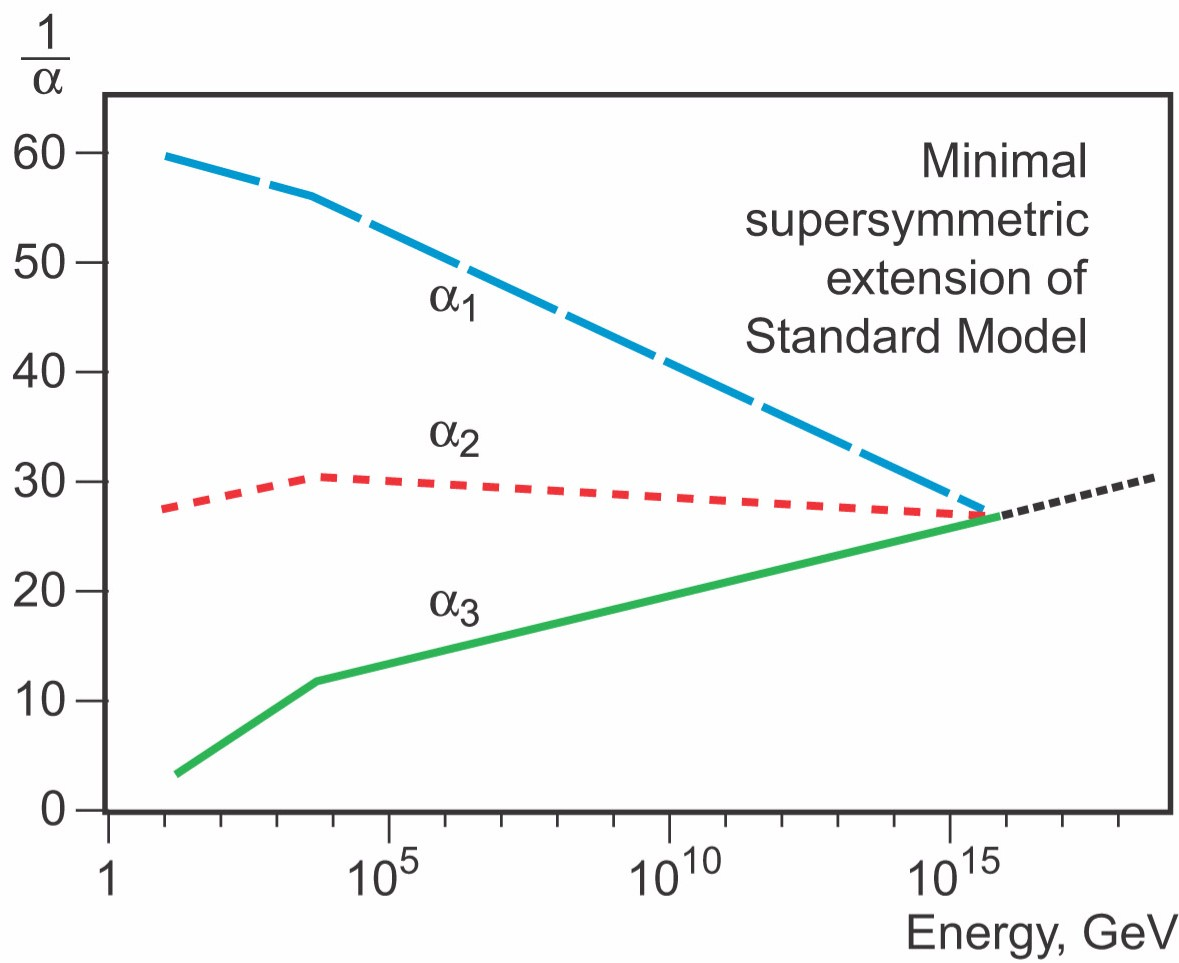
\includegraphics[width=\fullfig]{figures/unification_susy.jpg}
\caption{An approximation of the running of the coupling constants in the \ac{MSSM} up to the Planck scale~\cite{unification_plot}.}
\label{fig:unification_susy}
\end{figure}

The presence of R-parity in a \ac{SUSY} model also provides an explanation for dark matter.
The \ac{LSP}, as discussed in Section~\ref{sec:mssm}, is a massive, neutral, and stable particle as long as R-parity is conserved.
In the early universe, when the energy density was extremely high, \acp{LSP} could be spontaneously produced just as often as other particles like photons, and would result in a thermal equilibrium.
Then, as the universe cooled, the average energy would be too low to create additional \acp{LSP}, and they would be left behind and only interact with the remaining matter gravitationally, a process called freeze out.
Since those particles are stable, they would remain indefinitely. 
With the existence of an \ac{LSP} at around the \TeV scale, this process can explain the observed amount of dark matter in the universe.
A \ac{WIMP}, exactly what is proposed in the \ac{LSP}, provides the correct interaction rate to predict the currently observed ratio of dark matter to baryonic matter.

Together, this variety of solutions to existing problems provides strong theoretical support for the existence of \ac{SUSY} near the \TeV scale.
The \ac{LHC} is the first collider experiment to be able to probe into \TeV scale interactions, providing a new opportunity to search for this extension to the \ac{SM}.
A range of models have begun to be excluded with masses above 1 \TeV~\cite{pdg}, leading to a motivation to explore a wider variety of models with phenomena that may have been missed by the most direct search strategies.

\section{Simplified Models}

The \ac{MSSM} is just one example of a large suite of \ac{SUSY} models with similar results.
Each of those models can have hundreds of individual parameters that ultimately determine the masses and interactions of the supersymmetric particles.
To avoid this complexity in making experimental measurements, the analyses of high energy collisions often rely on simplified models.
These models focus on a single process predicted by a theory, and the observable parameters such as the mass of the particles and their lifetimes are controlled directly, rather than tuning the hundreds of underlying parameters.
This allows straightforward simulation of a specific event topology with control over the parameters that most directly influence the experimental signatures.

Experimental analyses use these models to search for new physics and to set limits on the production rates for a given type of process with working points of a few observable parameters.
As one example, a simplified model may specify pair production of gluinos where the free parameters are the mass of the gluino and the types and masses of the particles it can decay into.
The small number of parameters allows the phase space to be searched in a grid by simulating events with a few examples for the parameters and interpolating between them.
The resulting analysis can set cross sectional limits as a function of the simplified parameters, and this allows for an easy interpretation of the result in a number of \ac{SUSY} models.

\section{Long-Lived Particles}
\label{sec:llp_theory}

Some proposed \ac{SUSY} models can produce \acp{LLP} other than just the \ac{LSP}.
The most direct search strategies for \ac{SUSY} often assume that the various non-stable sparticles decay promptly, rather than propagating through some fraction of the detector.
Although the processes involved are very similar, the long-lifetime of the produced particles can lead to very different experimental signatures, and often require separate dedicated searches.
It is important to design and execute search strategies for \acp{LLP} in order to completely cover possible production of new physics. 

There are a several ways to generate long lifetimes for the massive \ac{SUSY} particles, depending on the specific model.
In examples like Spread Supersymmetry~\cite{spreadsusy} and Split Supersymmetry~\cite{split1,split2}, the introduction of a split between two mass scales suppresses the decay of gluinos.
In these and similar models, the squarks are much heavier than the gluino, where the mass scale of the squarks is roughly $10^6$ \GeV while the mass scale of the gluinos is roughly $10^3$ \GeV.
The gluino must decay through the production of a virtual squark, as shown in the diagram of Figure~\ref{fig:gluino_decay}.
The large mass of the squarks in the split models suppresses the decay rate, and can result in lifetimes of the order of 1 ns~\cite{spreadsusy}.

\begin{figure}
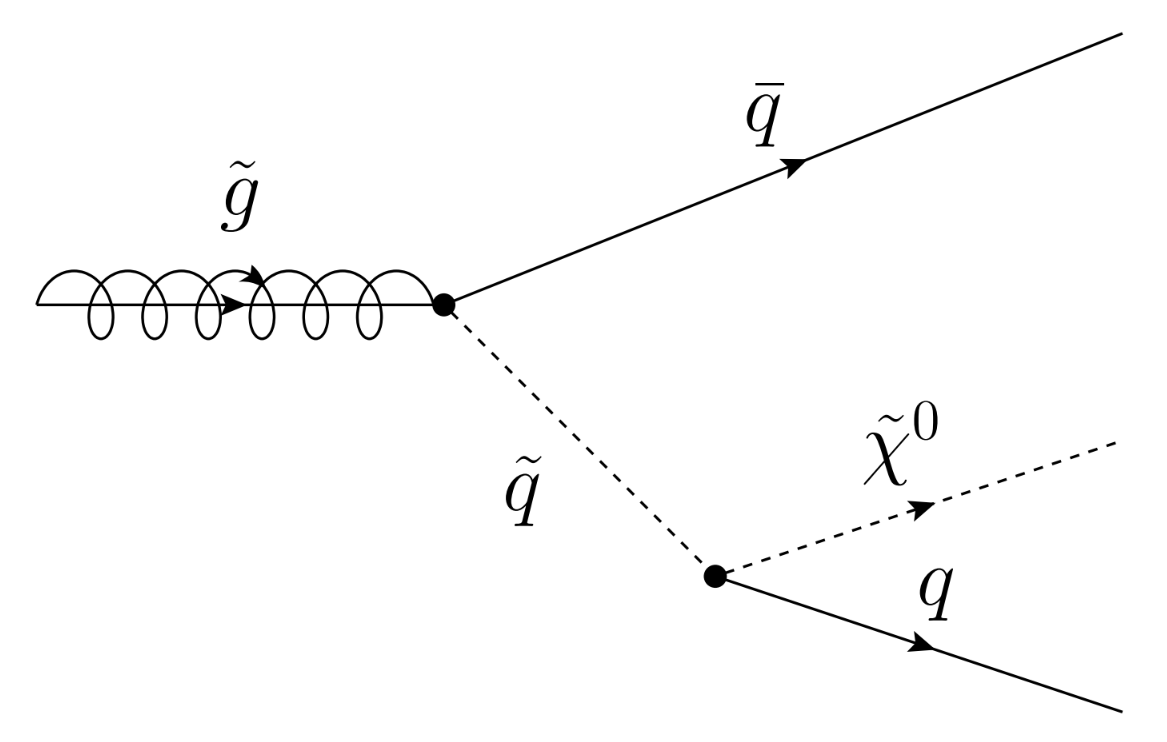
\includegraphics[width=\fullfig]{figures/gluino_decay.png}
\caption{The decay of a gluino to quarks and an \acs*{LSP}, which precedes through a squark.}
\label{fig:gluino_decay}
\end{figure}

Nearly degenerate particles can also result in long lifetimes, again by suppressing decay rates.
When a particle must decay to another particle with nearly the same mass, the phase space factor in the decay results in a low decay rate.
For example, a neutron has a lifetime of roughly fifteen minutes because its mass is so close to the proton.
Models which result in a nearly degenerate chargino and \ac{LSP} provide a long-lived chargino as well.

Again, because of the wide variety of models which can produce \acp{LLP} and the large number of parameters which determine their masses and lifetimes, the analysis presented here focuses on simplified models rather than assuming any particular underlying theory.
The models directly specify the decay mode of the \acp{LLP} as well as their masses and lifetimes, using a grid of values.
The results of searches using these simplified models can be interpreted over a very wide range of models that predict \acp{LLP}, even including non-supersymmetric extensions to the \ac{SM}.
